\chapter{Detailed Implementation}\label{ch:impl}

This chapter explains the implementation at the level of individual functions and the reasoning
behind them. Every excerpt is quoted from the committed source and the file and function are
named, so a reader can open the original. The complete source is supplied separately as
\code{COMPLETE\_SOURCE\_CODE\_AND\_EXPERIMENTS.zip}; the inventory is
Appendix~\ref{app:inventory}.

Three sections carry more weight than the rest and are the ones to read if time is short:
Section~\ref{sec:impl-cmd} on the command path, Section~\ref{sec:impl-guard} on the
configuration guard, and Section~\ref{sec:impl-drain} on the unbounded drain.

\section{Module map}

\begin{longtable}{@{}p{0.31\textwidth}p{0.61\textwidth}@{}}
\toprule
\textbf{File} & \textbf{Responsibility} \\
\midrule
\endhead
\code{smart\_home.ino} & The artefact under study. Pin definitions, timing constants, build
guards, the state machine, both cores' tasks, and the command path. 713 lines of code. \\
\code{authmac.h} & HMAC-SHA256 command authentication: tag computation and constant-time
comparison \\
\code{alertmsg.h} & Event record structure and serialisation \\
\code{wifi_guard.h} & Deauthentication frame counting and the detector threshold \\
\code{sensor_fusion.h} & Optional PIR and radar fusion; off in the evaluated configuration \\
\code{secrets.example.h} & Template for credentials and keys. The demo key it carries is
public by design, and the build refuses to use it with authentication enabled \\
\bottomrule
\end{longtable}

\section{Constants and the build configuration}

All timing and pin constants are \code{constexpr}, in one block, so that a reader auditing the
firmware's temporal behaviour can find every value in one place.

\begin{lstlisting}[style=cpp,caption={Timing constants, \code{smart\_home.ino}}]
constexpr uint32_t EXIT_DELAY_MS      = 10000;  // time to leave after pressing ARM
constexpr uint32_t ENTRY_DELAY_MS     = 10000;  // time to disarm after a trigger
constexpr uint32_t ALARM_DURATION_MS  = 30000;  // siren length, then system re-arms
constexpr uint32_t PIR_WARMUP_MS      = 10000;  // suits the simulator; 60000 on a real HC-SR501
constexpr uint32_t PIR_CONFIRM_MS     = 150;    // PIR must stay HIGH this long
constexpr uint32_t DEBOUNCE_MS        = 40;
constexpr uint32_t OLED_REFRESH_MS    = 250;
constexpr uint32_t STATUS_COPY_MS     = 500;    // loop -> network task snapshot rate
constexpr uint32_t HEARTBEAT_MS       = 30000;
constexpr uint32_t WIFI_RETRY_MS      = 15000;
constexpr uint32_t MQTT_RETRY_MS      = 5000;
\end{lstlisting}

\code{PIR\_WARMUP\_MS} carries a comment rather than a single value because the correct number
differs between the simulator and the physical sensor. Recording that in the source is
preferable to silently choosing one and misleading whoever deploys it.

\section{Data structures}

\begin{lstlisting}[style=cpp,caption={Core data structures, \code{smart\_home.ino}}]
enum class SysState : uint8_t { DISARMED, EXIT_DELAY, ARMED, ENTRY_DELAY, ALARM };
enum class Cmd      : uint8_t { ARM, DISARM, STATUS };

struct CmdMsg {   /* one entry in the command queue */
  Cmd      cmd;
  bool     authed;   /* the MAC verified */
  uint32_t ctr;      /* the counter carried by the command */
};
\end{lstlisting}

\code{CmdMsg} is deliberately small and contains no pointers. It is copied by value into a
FreeRTOS queue, so a command crossing the core boundary involves no shared allocation and no
lifetime question. The \code{authed} flag is set on core~0 after verification; core~1 trusts it
precisely because nothing else can write to that queue.

\section{Core 1: the safety loop}

\subsection{Input conditioning}

\code{readSensors()} samples the three input lines and applies two independent filters. The
button and the door switch are debounced over \code{DEBOUNCE\_MS}; the PIR is suppressed
entirely for \code{PIR\_WARMUP\_MS} after boot and then required to hold its indication for
\code{PIR\_CONFIRM\_MS}.

The two filters are different because the failure modes are different. A mechanical switch
chatters on contact, which debouncing addresses. A pyroelectric sensor produces spurious output
while its reference stabilises after power-up, and then occasional short pulses in normal
operation — a warm-up suppression and a confirmation window address those.

\subsection{The state machine}

\code{stepFsm()} implements the five-state machine of Chapter~\ref{ch:arch}. Its structure is a
switch on the current state, with time-based transitions compared against a stored entry
timestamp rather than counted down, so that a missed loop pass cannot lose time.

The armed state is written to non-volatile storage on every change through
\code{persistState()}, which satisfies FR6: a power interruption while armed leaves the system
armed.

\subsection{Output driving}

\code{driveOutputs()} is the only function that writes to the siren, the indicators or the
display. Concentrating output in one function means that a reader auditing when the siren can
sound has one place to look.

The buzzer driver handles an API change between arduino-esp32 2.x, which is channel-based, and
3.x, which is pin-based. The firmware supports both because both were evaluated.

\section{The command path}\label{sec:impl-cmd}

\subsection{Authentication on core 0}

The wire format is a verb, a counter and a truncated tag over both:
\[
\texttt{VERB}:\texttt{CTR}:\mathrm{hex}\bigl(\mathrm{HMAC\text{-}SHA256}(k,\ \texttt{"VERB:CTR"})[0{:}16]\bigr)
\]

Two design decisions are worth explaining. The tag is truncated to 128 bits
(\code{AUTH\_TAG\_BYTES = 16}) because a 256-bit tag in hexadecimal would double the wire
length for no practical security gain: the forgery probability against a 128-bit tag is
$2^{-128}$, which is far below any threshold that matters here. And the tag covers the
\emph{counter as well as the verb}, which is what prevents an adversary from taking a captured
command and incrementing its counter.

Comparison uses a constant-time routine in \code{authmac.h}. On a device of this kind a timing
side channel on tag comparison is a remote prospect, but constant-time comparison costs
nothing and removes the question.

\subsection{Dispatch on core 1}

\code{handleCommands()} runs on the safety core and is the only consumer of the command queue.

\begin{lstlisting}[style=cpp,caption={Command dispatch, \code{handleCommands()} in
\code{smart\_home.ino}},label={lst:handlecmd}]
static void handleCommands(uint32_t now) {
  CmdMsg m;
  for (int drained = 0;
       drained < CMD_DRAIN_PER_PASS && xQueueReceive(cmdQ, &m, 0) == pdTRUE;
       drained++) {
    // Marker from the network task for a command whose MAC did not verify.
    if (!m.authed && m.ctr == 0xFFFFFFFFu) { emitEvent("cmd_badmac", "remote"); continue; }

    if (m.authed) {
      // Reject a replay: the counter must strictly advance.
      if (m.ctr <= cmdCounter) { emitEvent("cmd_replay", "remote"); continue; }
      persistCounter(m.ctr);
    }
#if AUTH_COMMANDS
    else {
      // Authentication is required but this command was unsigned.
      emitEvent("cmd_unauth", "remote");
      continue;
    }
#endif
    const char* src = m.authed ? "remote_auth" : "remote";
    switch (m.cmd) {
      case Cmd::ARM:
        if (state == SysState::DISARMED) beginArm(src, now);
        else emitEvent("cmd_ignored", src);
        break;
      case Cmd::DISARM:
        if (m.authed || ALLOW_REMOTE_DISARM) {
          if (state != SysState::DISARMED) disarm(src, now);
          else emitEvent("cmd_ignored", src);
        } else {
          emitEvent("cmd_rejected", src);
        }
        break;
      case Cmd::STATUS:
        statusDirty = true;
        break;
    }
  }
}
\end{lstlisting}

Reading this block by block:

\begin{description}[leftmargin=1.6em,itemsep=4pt]
  \item[The loop header] is the bounded drain discussed in Section~\ref{sec:impl-drain}. The
        \code{0} timeout on \code{xQueueReceive} means the safety loop never waits for a
        command.
  \item[The \code{cmd\_badmac} marker] is how core~0 reports a verification failure without
        performing any dispatch itself. The sentinel counter \code{0xFFFFFFFF} distinguishes it
        from a genuine unsigned command.
  \item[The replay check] requires the counter to \emph{strictly} advance, and
        \code{persistCounter()} commits the new value \emph{before} the command is acted on.
        Committing afterwards would leave a window in which a power interruption between
        action and commit permits the same command to be replayed.
  \item[The \code{AUTH\_COMMANDS} branch] is where an unsigned command is refused when
        authentication is required. This is the clause the configuration guard of
        Section~\ref{sec:impl-guard} is supposed to protect.
  \item[The \code{DISARM} case] is the one that matters for security. A validly signed command
        proves the key holder sent it, so disarm is safe irrespective of
        \code{ALLOW\_REMOTE\_DISARM}. The disjunction exists for a deployment that uses TLS and
        a broker login without command signing — and the soundness of \emph{that} configuration
        is exactly what this project found to be unjustified.
  \item[\code{cmd\_ignored} versus \code{cmd\_rejected}] are distinguished deliberately: the
        first means a well-authorised command that does not apply in the current state, the
        second means a command that was not authorised. Conflating them would make the event
        log useless for exactly the analysis this project performed.
\end{description}

\section{The configuration guard}\label{sec:impl-guard}

\subsection{The defect}

The original guard permitted \code{ALLOW\_REMOTE\_DISARM} without \code{AUTH\_COMMANDS}
provided that TLS and a broker login were configured. The reasoning was that a deployment with
transport security and broker authentication has established who may publish.

The reasoning is unsound, and it is unsound for a structural reason rather than through an
oversight in the code. The broker terminates each client's TLS connection and re-originates
every message it forwards, so an arriving command carries no evidence of which client published
it. \code{MQTT\_HAS\_LOGIN} describes \emph{this device's own build}, not any publisher's
authority. One leaked credential — any credential permitted to publish on the command topic —
is therefore sufficient to disarm the alarm, and the guard compiled such a build without
complaint.

\subsection{The repair}

\begin{lstlisting}[style=cpp,caption={The corrected guard, \code{smart\_home.ino}},
                   label={lst:guard}]
#if ALLOW_REMOTE_DISARM && !AUTH_COMMANDS && !defined(ACKNOWLEDGE_UNAUTHENTICATED_DISARM)
#  error "ALLOW_REMOTE_DISARM without AUTH_COMMANDS 1 permits anyone who can publish to the \
command topic to switch the alarm off, and TLS plus a broker login does not prevent it (see \
docs/SECURITY_ANALYSIS.md). Set AUTH_COMMANDS 1, or define \
ACKNOWLEDGE_UNAUTHENTICATED_DISARM to accept that risk deliberately."
#endif
\end{lstlisting}

The repair removes the unsound inference rather than adding a mechanism. The transport test is
gone; what remains is a requirement for either command signing or an explicit acknowledgement
that the risk is being accepted. The latter exists because the research baseline must be able
to build the defective configuration in order to measure it — and it must do so deliberately.

Figure~\ref{fig:guard} shows both versions of the decision.

\begin{figure}[htbp]
\centering
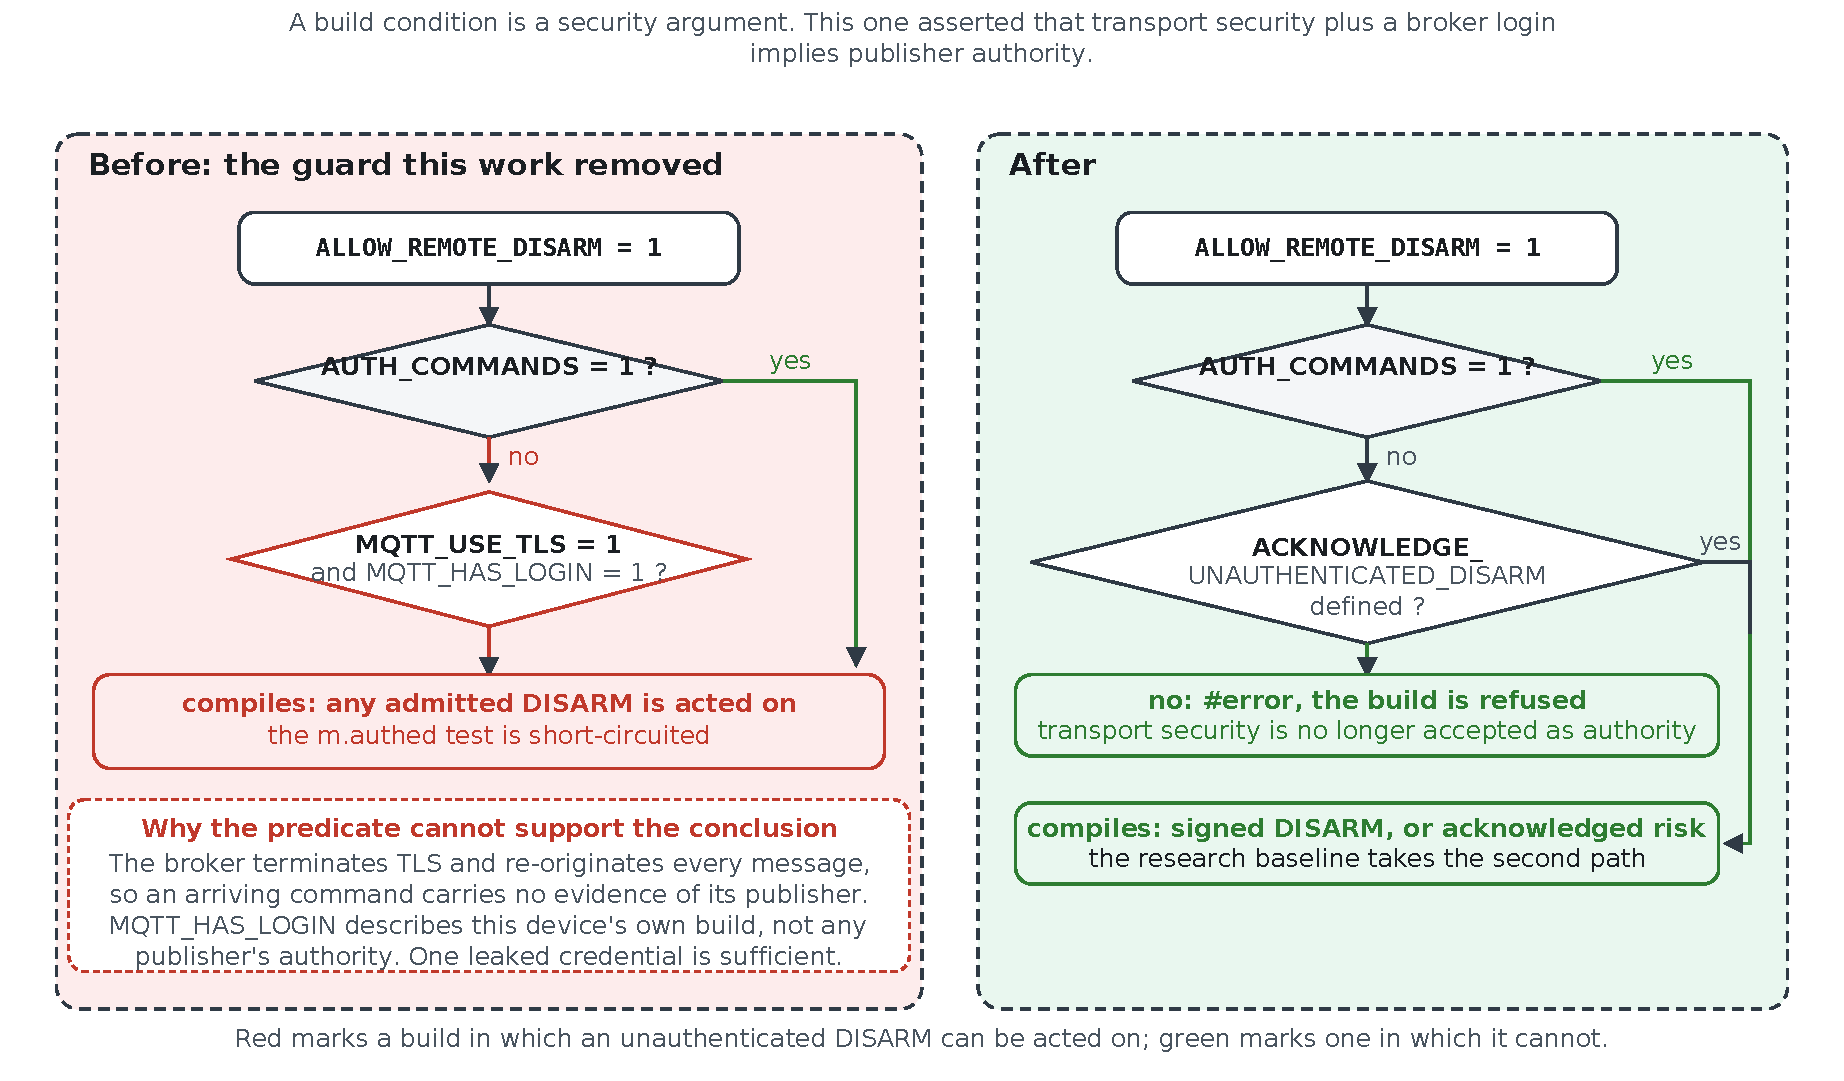
\includegraphics[width=\textwidth]{guard_decision.pdf}
\caption[Compile-guard comparison]{The defective guard and its repair, transcribed from the
preprocessor conditions. Both branches of the original reach the same outcome, which is the
defect: a signed build reaches it legitimately and an unsigned one through the unsound
transport test.}
\label{fig:guard}
\end{figure}

\subsection{A second guard: the published demo key}

A related defect was found and closed at the same time. The repository ships a
\code{secrets.example.h} whose demo command key is public by design. A build enabling
\code{AUTH\_COMMANDS} without replacing it would log every command as authenticated while any
reader of the repository could forge one.

\begin{lstlisting}[style=cpp,caption={Refusing the published key, \code{smart\_home.ino}}]
#if AUTH_COMMANDS && CMD_KEY_IS_DEMO
#  error "AUTH_COMMANDS 1 requires a real SECRET_CMD_KEY in secrets.h. The fallback key is \
published in this repository, so a command signed with it is forgeable by any reader."
#endif
\end{lstlisting}

Authentication that verifies against a published key is not authentication. The build now
refuses rather than producing a binary that reports false assurance.

\section{Response-time analysis and the unbounded drain}\label{sec:impl-rt}

\subsection{The decomposition}

The response time of the safety loop decomposes into the loop's own execution, interference
from the network core, blocking on shared resources, and residual hardware contention. Three of
the four are settled by construction.

\begin{description}[leftmargin=1.8em,itemsep=4pt]
  \item[Blocking is identically zero.] The safety loop acquires the status mutex with timeout
        \code{0} and proceeds without it on failure (Listing~\ref{lst:mutex}). It never waits,
        so no priority inversion and no blocking term exists.
  \item[Queue interference is bounded.] Both queues are bounded, both enqueues are
        non-blocking, and the event queue drops its oldest entry when full rather than making
        the producer wait.
  \item[Scheduling interference is bounded by core affinity.] The network task is pinned to
        core~0 and the safety loop runs on core~1, so the network task cannot be scheduled
        ahead of the safety loop.
  \item[Residual hardware contention cannot be settled analytically.] Contention for the
        memory bus, the caches and the interrupt controller remains, and it depends on the
        silicon and on a closed-source radio driver. This is the single composite term that
        requires measurement, and it is why Appendix~\ref{app:hardware} exists.
\end{description}

\subsection{The defect the analysis exposed}\label{sec:impl-drain}

Performing that decomposition revealed something the author had not been looking for. The
command drain was an unbounded loop:

\begin{lstlisting}[style=cpp,caption={The defective drain, before the repair}]
/* BEFORE -- no static bound on the loop's own execution time */
while (xQueueReceive(cmdQ, &m, 0) == pdTRUE) {
    /* ... dispatch ... */
}
\end{lstlisting}

The safety loop therefore had no static bound on its own execution time. Core~0 can enqueue
while core~1 dequeues, and in the default build — with \code{AUTH\_COMMANDS} disabled —
enqueueing costs only a parse, with no HMAC computation to throttle the producer. The loop
would still terminate in practice, but only through a probabilistic argument about relative
costs. That is not an acceptable basis for the one code path whose timing the entire design
exists to protect.

\begin{lstlisting}[style=cpp,caption={The repaired bound and its assertions,
\code{smart\_home.ino}},label={lst:drain}]
// Capacity of the command queue, and the bound on how many are drained per loop pass.
static constexpr int CMD_Q_LEN = 4;

// The bound equals the queue capacity, so a full queue still drains in a single pass;
// anything arriving during the pass waits for the next one, at most one loop period.
static constexpr int CMD_DRAIN_PER_PASS = CMD_Q_LEN;

static_assert(CMD_DRAIN_PER_PASS == CMD_Q_LEN,
              "the per-pass drain bound must equal the command queue capacity: smaller leaves "
              "work queued for an unbounded number of passes, larger makes the loop's worst "
              "case depend on arrival rate again");
static_assert(CMD_DRAIN_PER_PASS > 0, "a non-positive drain bound would never dequeue");
\end{lstlisting}

The bound equals the queue capacity, which is the only value that works: a smaller bound leaves
work queued for an unbounded number of passes, and a larger one makes the loop's worst case
depend on arrival rate again — reintroducing the original defect. The two static assertions
exist because deriving one constant from the other is not sufficient protection: a later change
could redefine either independently, and the response-time bound holds only while the
relationship between them does. Asserting the relationship is preferable to trusting a comment.

\subsection{Why this defect is the most instructive result in the project}

The unbounded drain had survived:

\begin{itemize}[leftmargin=1.6em,itemsep=3pt]
  \item 129 host tests;
  \item 3,000,000 fuzzing iterations under AddressSanitizer and UndefinedBehaviorSanitizer;
  \item 9,600 adversarial trials, including sustained flooding at up to 20,000 messages per
        second;
  \item exhaustive model checking of both specifications.
\end{itemize}

Every one of those techniques exercises a \emph{running system}, and in every execution the loop
terminated. None of them asks whether the loop's termination is \emph{bounded}, because that is
a question about the program's design rather than about any particular execution. An analytical
method costing an afternoon found what several million executions did not.

\section{The network task}

\code{networkTask()} is a conventional reconnect loop. Its structure is a state check followed
by the appropriate action, with each retry governed by its own interval constant so that a
failing Wi-Fi connection does not cause an MQTT reconnect storm.

Error handling throughout is by \emph{omission rather than exception}: a failed publish is
retried on the next pass, a failed snapshot acquisition is skipped, and a failed NTP
synchronisation leaves timestamps uncorrected. None of these conditions can propagate into the
safety core, because the only channel into it carries verified commands.

\section{Event reporting}

\code{emitEvent()} enqueues a structured event on \code{eventQ}, which the network task drains
and publishes as JSON with a sequence number. Events are published oldest first.

The queue drops its \emph{oldest} entry when full rather than refusing the newest. This is the
correct choice for a safety device: during an incident the most recent events are the
informative ones, and under no circumstances may the safety loop be made to wait for a
telemetry consumer.

The event vocabulary is deliberately specific — \code{cmd\_badmac}, \code{cmd\_unauth},
\code{cmd\_replay}, \code{cmd\_rejected}, \code{cmd\_ignored} — and the ablation measurements in
Chapter~\ref{ch:results} are counted from these names. A coarser vocabulary would have made
those measurements impossible.

\section{Resource cost}\label{sec:impl-cost}

Table~\ref{tab:rep-build} in Chapter~\ref{ch:tools} gives flash and RAM for both framework
versions. The firmware occupies 60.5\% of flash under arduino-esp32 2.0.17 and 73.9\% under
3.3.12, with RAM at roughly 14--15\% in both cases. The headroom is adequate but not generous,
which is one reason no additional mechanism was introduced where the repair of an existing one
would do.

\section{How the implementation was tested}

\begin{longtable}{@{}p{0.29\textwidth}p{0.63\textwidth}@{}}
\toprule
\textbf{Component} & \textbf{How it is tested} \\
\midrule
\endhead
State machine & \code{tests/host/test\_firmware.cpp}: transition assertions for every state
pair, plus 19,529 observed transitions checked against the TLA+ relation \\
Input conditioning & host tests for debounce behaviour and the PIR confirmation window \\
Command authentication & differential test D1 in \code{experiments/test\_harness.py}: the
firmware's HMAC payload format is compared against an independent implementation for three
counter values including \code{0xFFFFFFFF} \\
Replay rejection & ablation arms measuring whether captured material yields an accepted
command \\
Build guards & three negative tests that require a defective configuration to \emph{fail} to
compile \\
Drain bound & two \code{static\_assert}s, so a violation is a compile error rather than a
runtime surprise \\
Queue discipline & the \code{Isolation} TLA+ model, checked exhaustively with no fairness
assumption on the network task \\
Command parser & 3,000,000 fuzzing iterations under both sanitizers \\
\bottomrule
\end{longtable}

The three negative build-guard tests deserve a note. A test that asserts a correct build
compiles tells you very little; a test that asserts a \emph{defective} build fails to compile is
what demonstrates the guard is doing anything at all. The same principle governs the formal
verification in Chapter~\ref{ch:formal} and the corpus rule controls in
Section~\ref{sec:res-corpus}.
